\documentclass[aspectratio=169]{beamer}

% ============================================================
%  Introduction to ARM Cortex-M Microprocessors
%  Chapter 10 — Timers, Timing and PWM
%  Munim Zabidi, Faculty of Electrical Engineering, UTM
% ============================================================

\usepackage[utf8]{inputenc}
\usepackage{listings}
\usepackage{xcolor}
\usepackage{amsmath}
\usepackage{tikz}
\usetikzlibrary{arrows.meta, positioning}

% ---------- Theme ----------
\usetheme{default}
\definecolor{utmgray}{RGB}{89,89,89}
\definecolor{utmgreen}{RGB}{58,110,86}
\definecolor{utmcream}{RGB}{253,251,235}
\setbeamercolor{frametitle}{bg=utmgray, fg=white}
\setbeamercolor{title}{bg=utmgray, fg=white}
\setbeamercolor{structure}{fg=utmgreen}
\setbeamercolor{block title}{bg=utmgray, fg=white}
\setbeamercolor{block body}{bg=utmcream}
\setbeamertemplate{navigation symbols}{}
\setbeamertemplate{footline}{%
  \hbox{\begin{beamercolorbox}[wd=\paperwidth,ht=2.5ex,dp=1ex,leftskip=1em,rightskip=1em]{structure}
    {\scriptsize \copyright\ Mun\'im Zabidi \hfill \insertframenumber}
  \end{beamercolorbox}}
}

% ---------- Code listings style ----------
\lstdefinestyle{cstyle}{
  language=C,
  basicstyle=\ttfamily\scriptsize,
  keywordstyle=\color{blue!70!black},
  commentstyle=\color{utmgreen},
  stringstyle=\color{orange!70!black},
  numbers=none,
  breaklines=true,
  showstringspaces=false,
  backgroundcolor=\color{black!4},
  frame=single,
  rulecolor=\color{black!20},
  tabsize=2,
}
\lstset{style=cstyle}

\title{Timers, Timing and PWM}
\subtitle{Introduction to ARM Cortex-M Microprocessors --- Chapter 10}
\author{Mun\'im Zabidi}
\institute{Faculty of Electrical Engineering, Universiti Teknologi Malaysia}
\date{}

\begin{document}

% ------------------------------------------------------------
\begin{frame}
  \titlepage
\end{frame}

% ------------------------------------------------------------
\begin{frame}{Table of Contents}
  \tableofcontents
\end{frame}

% ============================================================
\section{Why This Matters}
% ============================================================

\begin{frame}{Why This Chapter Matters}
  Every program so far has used \texttt{delay\_ms()} --- a loop that counts
  down and does nothing. It is wrong in three ways: its timing changes if
  you change the compiler optimization level or the clock frequency, it
  consumes 100\% of the CPU while waiting, and it cannot be calibrated
  accurately. A hardware timer solves all three. It counts independently
  of the processor, generates precise intervals, measures elapsed time
  exactly, and produces the pulse-width modulated signals that dim LEDs
  and drive motors.
\end{frame}

\begin{frame}{Objectives}
  After completing this chapter, you should be able to:
  \begin{enumerate}
    \item Explain how a prescaler and auto-reload register set a timer's period.
    \item Calculate the prescaler and reload values needed for a required timing interval.
    \item Configure a general-purpose timer for periodic update interrupts.
    \item Use SysTick to maintain a millisecond system time base.
    \item Select the correct alternate function number to route a pin to a timer channel.
    \item Calculate PWM frequency and duty cycle, and configure a timer output compare channel to generate one.
    \item Apply PWM to control LED brightness and motor speed.
  \end{enumerate}
\end{frame}

% ============================================================
\section{Why Software Delays Fail}
% ============================================================

\begin{frame}[fragile]{Three Things Wrong With \texttt{delay\_ms()}}
\begin{columns}[T]
\column{0.5\textwidth}
\begin{lstlisting}
void delay_ms(int n) {
  for (volatile int i = 0;
       i < n * 4000; i++) ;
}
\end{lstlisting}
\column{0.5\textwidth}
\begin{enumerate}
  \item Its timing changes with the compiler optimisation level and the clock frequency
  \item It consumes 100\% of the CPU while waiting
  \item It cannot be interrupted accurately --- any ISR that fires makes the delay longer
\end{enumerate}
\end{columns}
\vspace{1em}
\begin{block}{A timer is a counter in hardware}
It runs independently of the processor, at a rate you configure. It does
not care what the CPU is doing, what the optimiser did, or how many
interrupts fired. That is what makes it a clock rather than a guess.
\end{block}
\end{frame}

% ============================================================
\section{Timer Architecture}
% ============================================================

\begin{frame}{Prescaler and Auto-Reload}
\centering
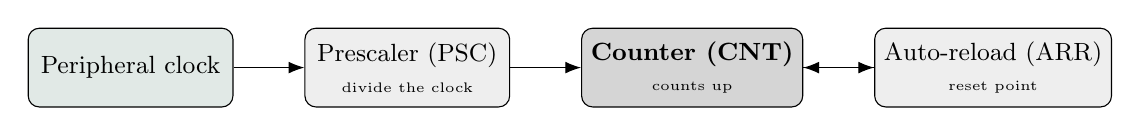
\begin{tikzpicture}[
  box/.style={draw, rounded corners, minimum height=1cm, minimum width=2.6cm, align=center, font=\small},
  arr/.style={-{Latex[length=2mm]}}
]
  \node[box, fill=utmgreen!15] (clk)  {Peripheral clock};
  \node[box, right=0.9cm of clk, fill=utmgray!10] (psc)  {Prescaler (PSC)\\ \tiny divide the clock};
  \node[box, right=0.9cm of psc, fill=utmgray!25] (cnt)  {\textbf{Counter (CNT)}\\ \tiny counts up};
  \node[box, right=0.9cm of cnt, fill=utmgray!10] (arr)  {Auto-reload (ARR)\\ \tiny reset point};

  \draw[arr] (clk) -- (psc);
  \draw[arr] (psc) -- (cnt);
  \draw[arr] (arr) -- (cnt);
  \draw[arr] (cnt) -- (arr);
\end{tikzpicture}

\vspace{1em}
\[
f_{\text{event}} = \frac{f_{\text{CK}}}{(\text{PSC}+1)\times(\text{ARR}+1)}
\]

\vspace{0.5em}
{\small The $+1$ is because a value of 0 means ``divide by 1'' --- a counter
that reloads at 0 still counts one tick.}
\end{frame}

\begin{frame}[fragile]{A Timing Calculation}
\begin{columns}[T]
\column{0.5\textwidth}
\textbf{Required}\\
A 1\,Hz interrupt from a 16\,MHz clock.

\vspace{0.5em}
\textbf{Choose a prescaler}\\
PSC = 15999 divides 16\,MHz down to 1\,kHz --- a convenient 1\,ms tick.

\column{0.5\textwidth}
\textbf{Then the reload value}\\
ARR = 999 gives 1000 ticks = 1\,s.

\[
\text{Check: } \frac{16{,}000{,}000}{16000 \times 1000} = 1\,\text{Hz}
\]

\begin{lstlisting}
TIM2->PSC = 15999;
TIM2->ARR = 999;
\end{lstlisting}
\end{columns}

\vspace{1em}
\begin{block}{Why choose PSC first}
Both registers are 16-bit, so neither can exceed 65535. Pick the prescaler
to give a convenient tick --- 1\,ms or 1\,\textmu s --- then the reload
value is just the number of ticks you want.
\end{block}
\end{frame}

\begin{frame}[fragile]{A Periodic Timer Interrupt}
\begin{lstlisting}
RCC->APB1ENR |= (1U << 0);       // TIM2 clock
TIM2->PSC = 15999;                // 16 MHz -> 1 kHz
TIM2->ARR = 999;                  // 1000 ticks -> 1 Hz
TIM2->DIER |= (1U << 0);          // update interrupt enable
TIM2->CR1  |= (1U << 0);          // start counting
NVIC_EnableIRQ(TIM2_IRQn);

void TIM2_IRQHandler(void)
{
    if (TIM2->SR & (1U << 0)) {   // update flag?
        TIM2->SR &= ~(1U << 0);   // clear it
        GPIOA->ODR ^= (1U << 5);
    }
}
\end{lstlisting}
{\small The CPU is now free between interrupts --- it can sleep, or do
real work, and the LED still blinks at exactly 1\,Hz.}
\end{frame}

\begin{frame}[fragile]{SysTick --- The System Time Base}
\begin{columns}[T]
\column{0.5\textwidth}
\begin{itemize}
  \item A 24-bit down-counter built into the \textbf{core}, not the vendor's peripherals.
  \item Present on \textbf{every} Cortex-M, at the same address --- so code using it is portable.
  \item Normally configured for a 1\,ms tick.
\end{itemize}
\begin{lstlisting}
SysTick_Config(SystemCoreClock / 1000);
\end{lstlisting}
\column{0.5\textwidth}
\begin{lstlisting}
volatile uint32_t ticks = 0;

void SysTick_Handler(void)
{
    ticks++;
}

uint32_t millis(void)
{
    return ticks;
}
\end{lstlisting}
\end{columns}

\vspace{0.5em}
\begin{block}{This is what replaces \texttt{delay\_ms()}}
Instead of \emph{waiting}, record when something last happened and check
whether enough time has passed. That is the non-blocking pattern
Chapter 14 builds a whole system from.
\end{block}
\end{frame}

% ============================================================
\section{Alternate Functions}
% ============================================================

\begin{frame}{Routing a Pin to a Peripheral}
\centering
\small
\begin{tabular}{r l}
AF0  & (system) \\
AF1  & (TIM1/TIM2) \\
AF2  & (TIM3..5) \\
AF3  & (TIM8..11, CEC) \\
AF4  & (I2C1..4, CEC) \\
AF5  & (SPI1/2/3/4) \\
AF6  & (SPI2/3/4, SAI1) \\
AF7  & (SPI2/3, USART1..3, UART5, SPDIF-IN) \\
AF8  & (SPI2/3, USART1..3, UART5, SPDIF-IN) \\
AF9  & (CAN1/2, TIM12..14, QUADSPI) \\
AF10 & (SAI2, QUADSPI, OTG\_HS, OTG\_FS) \\
AF11 & \\
AF12 & (FMC, SDIO, OTG\_HS$^{(1)}$) \\
AF13 & (DCMI) \\
AF14 & \\
AF15 & (EVENTOUT) \\
\end{tabular}

\vspace{0.5em}
{\small A pin can serve several peripherals. \texttt{MODER} set to
\texttt{10} selects alternate-function mode; \texttt{AFR} then chooses
which of up to sixteen functions.}
\end{frame}

\begin{frame}[fragile]{Selecting the Function Number}
\begin{itemize}
  \item Four bits per pin, so \texttt{AFR[0]} covers pins 0--7 and \texttt{AFR[1]} covers pins 8--15.
  \item For pin $n \ge 8$ the shift is $(n-8)\times 4$.
\end{itemize}

\begin{lstlisting}
// PA5 -> TIM2_CH1 is AF1
GPIOA->MODER &= ~(3U << 10);
GPIOA->MODER |=  (2U << 10);

GPIOA->AFR[0] |= (1U << (5*4));
\end{lstlisting}

{\small The function numbers are in the \textbf{datasheet}, not the
reference manual --- a distinction that costs people an afternoon.}
\end{frame}

% ============================================================
\section{PWM}
% ============================================================

\begin{frame}{Pulse Width Modulation}
\centering
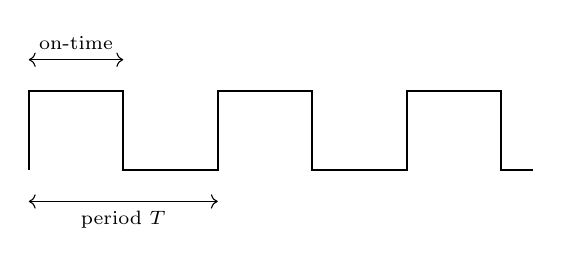
\begin{tikzpicture}[scale=1]
  \draw[thick] (0,0) -- (0,1) -- (1.2,1) -- (1.2,0) -- (2.4,0) -- (2.4,1) -- (3.6,1) -- (3.6,0) -- (4.8,0) -- (4.8,1) -- (6,1) -- (6,0) -- (6.4,0);
  \draw[<->] (0,1.4) -- (1.2,1.4) node[midway, above, font=\scriptsize]{on-time};
  \draw[<->] (0,-0.4) -- (2.4,-0.4) node[midway, below, font=\scriptsize]{period $T$};
\end{tikzpicture}

\vspace{1em}
\[
\text{duty cycle} = \frac{\text{on-time}}{T}
\qquad
f_{\text{PWM}} = \frac{f_{\text{CK}}}{(\text{PSC}+1)(\text{ARR}+1)}
\]

\vspace{0.5em}
\begin{block}{A digital pin producing an analog effect}
The pin is only ever fully on or fully off --- but switch it fast enough
and an LED looks dimmed, a motor runs slower, a heater delivers less
power. The average is what the load responds to.
\end{block}
\end{frame}

\begin{frame}[fragile]{Configuring PWM}
\begin{lstlisting}
TIM2->PSC  = 15;      // 16 MHz -> 1 MHz
TIM2->ARR  = 999;     // 1 MHz / 1000 = 1 kHz PWM
TIM2->CCR1 = 250;     // 250/1000 = 25% duty

TIM2->CCMR1 |= (6U << 4);  // PWM mode 1 on channel 1
TIM2->CCMR1 |= (1U << 3);  // preload enable
TIM2->CCER  |= (1U << 0);  // enable the output
TIM2->CR1   |= (1U << 0);  // start
\end{lstlisting}

\begin{block}{ARR sets the frequency, CCR sets the duty}
Change \texttt{CCR1} at any time and the duty cycle changes on the next
cycle --- no glitch, because the preload register updates only at the
reload point. That is what makes smooth dimming possible.
\end{block}

{\small A higher PWM frequency is less visible but wastes more switching
energy. For LEDs, 1\,kHz is comfortably above flicker perception.}
\end{frame}

% ============================================================
\section{More Code Examples}
% ============================================================

\begin{frame}[fragile]{The Bad \texttt{delay\_ms()} --- For Comparison}
\begin{lstlisting}
void delay_ms_bad(int n)
{
    for (volatile int i = 0; i < n * 4000; i++)
        ;
    /* Wrong in three ways: drifts with optimisation level
       and clock frequency, burns 100% CPU, and any ISR that
       fires makes it longer than requested. Do not use this
       in real designs. */
}
\end{lstlisting}
\end{frame}

\begin{frame}[fragile]{A Proper \texttt{delay\_ms()} --- Built on SysTick}
\begin{lstlisting}
static volatile uint32_t systick_ms = 0;

void SysTick_Handler(void) { systick_ms++; }

void systick_init(uint32_t core_clock_hz)
{
    SysTick_Config(core_clock_hz / 1000U); // 1 ms tick
}

uint32_t millis(void) { return systick_ms; }

// Blocking, but exact regardless of compiler optimisation:
// it counts real elapsed ticks, not a fixed loop count.
void delay_ms(uint32_t n)
{
    uint32_t start = millis();
    while ((millis() - start) < n) {
        __asm volatile ("wfi");  // sleep between ticks
    }
}
\end{lstlisting}
\end{frame}

\begin{frame}[fragile]{An Alternative: \texttt{delay\_ms()} on a General-Purpose Timer}
\begin{lstlisting}
void tim2_delay_init(void)
{
    RCC->APB1ENR |= (1U << 0);  // TIM2 clock enable
    TIM2->PSC = 15999;          // 16 MHz -> 1 kHz
    TIM2->ARR = 0xFFFF;         // free-running
    TIM2->CR1 |= (1U << 0);     // start counting
}

void delay_ms_tim2(uint32_t n)
{
    TIM2->CNT = 0;
    while (TIM2->CNT < n)
        ;
}
\end{lstlisting}
{\small Useful when SysTick is already claimed by an RTOS, and the
mechanism is the same prescaler/auto-reload arithmetic from earlier in
this chapter.}
\end{frame}

\begin{frame}[fragile]{The Non-Blocking Pattern (Preview of Chapter 14)}
\begin{lstlisting}
typedef struct {
    uint32_t last_ms;
    uint32_t period_ms;
} periodic_task_t;

int task_due(periodic_task_t *t)
{
    if ((millis() - t->last_ms) >= t->period_ms) {
        t->last_ms += t->period_ms;  // schedule next, no drift
        return 1;
    }
    return 0;
}

// Example: blink an LED every 500 ms without ever blocking
void non_blocking_blink_demo(void)
{
    static periodic_task_t blink = { .last_ms = 0, .period_ms = 500 };
    for (;;) {
        if (task_due(&blink)) GPIOA->ODR ^= (1U << 5);
        /* ... other work happens here every loop iteration ... */
    }
}
\end{lstlisting}
\end{frame}

\begin{frame}[fragile]{PWM Duty-Cycle Helper}
\begin{lstlisting}
void pwm_init_tim2_ch1(uint32_t psc, uint32_t arr)
{
    RCC->APB1ENR |= (1U << 0);
    TIM2->PSC = psc;
    TIM2->ARR = arr;
    TIM2->CCR1 = 0;                // start at 0% duty
    TIM2->CCMR1 |= (6U << 4);      // PWM mode 1, channel 1
    TIM2->CCMR1 |= (1U << 3);      // preload enable
    TIM2->CCER  |= (1U << 0);      // enable output
    TIM2->CR1   |= (1U << 0);      // start
}

// percent: 0-100
void pwm_set_duty_percent(uint8_t percent)
{
    if (percent > 100) percent = 100;
    uint32_t arr = TIM2->ARR;
    TIM2->CCR1 = ((uint32_t)percent * (arr + 1)) / 100U;
}
\end{lstlisting}
\end{frame}

\begin{frame}[fragile]{Example: A Breathing LED, Non-Blocking}
\begin{lstlisting}
void led_breathe_demo(void)
{
    static periodic_task_t step = { .last_ms = 0, .period_ms = 20 };
    static int duty = 0;
    static int dir  = 1;

    if (task_due(&step)) {
        duty += dir;
        if (duty >= 100 || duty <= 0) dir = -dir;
        pwm_set_duty_percent((uint8_t)duty);
    }
}
\end{lstlisting}
{\small Every 20\,ms the duty cycle steps by one percentage point up or
down, driven entirely by \texttt{task\_due()} --- no blocking call
anywhere in the loop.}
\end{frame}

\begin{frame}[fragile]{Design-Challenge Skeleton: One Time Base, Three Tasks}
\begin{lstlisting}
static periodic_task_t sensor_task  = { .last_ms=0, .period_ms=10   };
static periodic_task_t display_task = { .last_ms=0, .period_ms=100 };
static periodic_task_t log_task     = { .last_ms=0, .period_ms=1000};

void read_sensor(void)    { /* ... */ }
void update_display(void) { /* ... */ }
void write_log(void)      { /* ... */ }

void scheduler_loop(void)
{
    for (;;) {
        if (task_due(&sensor_task))  read_sensor();
        if (task_due(&display_task)) update_display();
        if (task_due(&log_task))     write_log();
    }
}
\end{lstlisting}
{\small One SysTick-driven \texttt{millis()} schedules the sensor
(10\,ms), display (100\,ms) and log (1\,s) tasks from a single
interrupt source, without drift.}
\end{frame}

% ============================================================
\section{Summary}
% ============================================================

\begin{frame}{Summary}
\begin{itemize}
  \item A software delay is wrong three ways: it depends on the \textbf{optimiser} and \textbf{clock}, it burns the \textbf{whole CPU}, and interrupts \textbf{stretch} it.
  \item A timer is a \textbf{hardware counter}: $f = f_{\text{CK}}/((\text{PSC}{+}1)(\text{ARR}{+}1))$.
  \item Choose \textbf{PSC} for a convenient tick, then \textbf{ARR} is the number of ticks.
  \item \textbf{SysTick} is in the core, identical on every Cortex-M, and is what a portable \texttt{millis()} is built on.
  \item An \textbf{alternate function} needs \texttt{MODER = 10} \emph{and} the right number in \texttt{AFR} --- four bits per pin.
  \item \textbf{PWM}: \texttt{ARR} sets the frequency, \texttt{CCR} sets the duty cycle. A digital pin produces an analog effect.
  \item The \textbf{non-blocking pattern} (\texttt{millis()} + \texttt{task\_due()}) replaces \texttt{delay\_ms()} in real designs and scales to any number of periodic tasks.
\end{itemize}

\vspace{0.5em}
\begin{block}{Next: Chapter 11 --- ADC and Analog Interfacing}
You can produce an analog effect. Next: measuring a real one.
\end{block}
\end{frame}

% ============================================================
\section{Design Challenge}
% ============================================================

\begin{frame}{Design Challenge \small (To be worked on paper, before any code)}
\begin{block}{The brief}
A system must perform three periodic tasks: read a sensor every 10\,ms,
update a display every 100\,ms, and write a log entry every 1\,s.
\end{block}

\small
Design the timing structure using a single hardware time base. Specify
the timer's PSC and ARR values for a 16\,MHz clock, and show how one
interrupt can schedule all three tasks without drift. Then determine
what happens if the log write takes 40\,ms, identify which requirement
breaks first, and give two different ways to fix it --- one that
changes the schedule and one that changes the architecture.

\vspace{0.5em}
\textbf{Extension --- a listening device.} Now add a fourth activity to
the same processor: sampling a microphone at 16\,kHz for keyword
spotting, as in audio timing. On paper, determine whether the system
above can still meet all its deadlines. Produce a cycle budget at
16\,MHz showing what fraction of the processor the sampling ISR alone
consumes; decide which of the four activities may be delayed and which
may not, and justify the ranking in terms of what breaks when each one
slips. State where the audio buffer lives and how the main loop knows a
window is ready without racing the ISR. Finally, identify the one
activity in the original three that is now unsafe to leave as written,
and say what you would change about it --- without adding a second
processor.
\end{frame}

\begin{frame}
  \centering
  \Huge Questions?

  \vspace{1em}
  \large Introduction to ARM Cortex-M Microprocessors --- Chapter 10
\end{frame}

\end{document}
